\section{Neural Computing}
The main area of my focus for this project is in
Artificial Neural Networks (ANN). This is because extensive research has been carried out into Convolutional Neural Networks (CNNs) which are based on ANNs.
\tocless\subsection{Artificial Neural Networks}
An Artificial Neural Network is a bio-inspired system that is used to model the human brain in how it learns from experience.
ANNs were first introduced in 1943 and were studied until the 1960's when the concept was shelved and revived gain in the 1980's \parencite{handsOnML}.
The ANN uses this model to build a very complex web of connected units called
artificial neurons.
These neurons are connected by certain weights which determines the processing
capacity of the network and these weights are created by learning a
dataset \parencite{malachy}.
A neuron has a set of inputs that take in a value, sometimes from network outputs
and produce a single result or classification.

As stated above, an ANN is bio-inspired from biological neurons \parencite{handsOnML}.
Biological neurons are cells located in animal's brains.
These neurons receive signals (electrical impulses) from other neurons and fires their own signal thereafter.
While an individual neuron is very simple, millions of these neurons working together can result in very complex computations.
From this, an artificial neuron was proposed through a simple model which had a binary input (1 or more) and a single binary output.


Before Convolution Neural Networks can be explored, which are vital to image
processing, the perceptron learning algorithm, the multi-layer perceptron, backpropagation must be analysed.

\tocless\subsubsection{Perceptron Learning - Artificial Neuron}
In our ANN, a perceptron is an artificial neuron.
It is called an artificial neuron because it is a bio-inspired neuron which models
a neuron in the human brain in terms of inputs and output.

In perceptron learning, we can take two inputs which are put towards an
activation function with a bias attached as seen in Figure \ref{fig:perceptron}.
These inputs are multiplied by the weights that connect the input to the
activation function and depending on the result, the activation function may
fire an output. These inputs are either 1 or -1.

\begin{figure}[h]
	\centering
     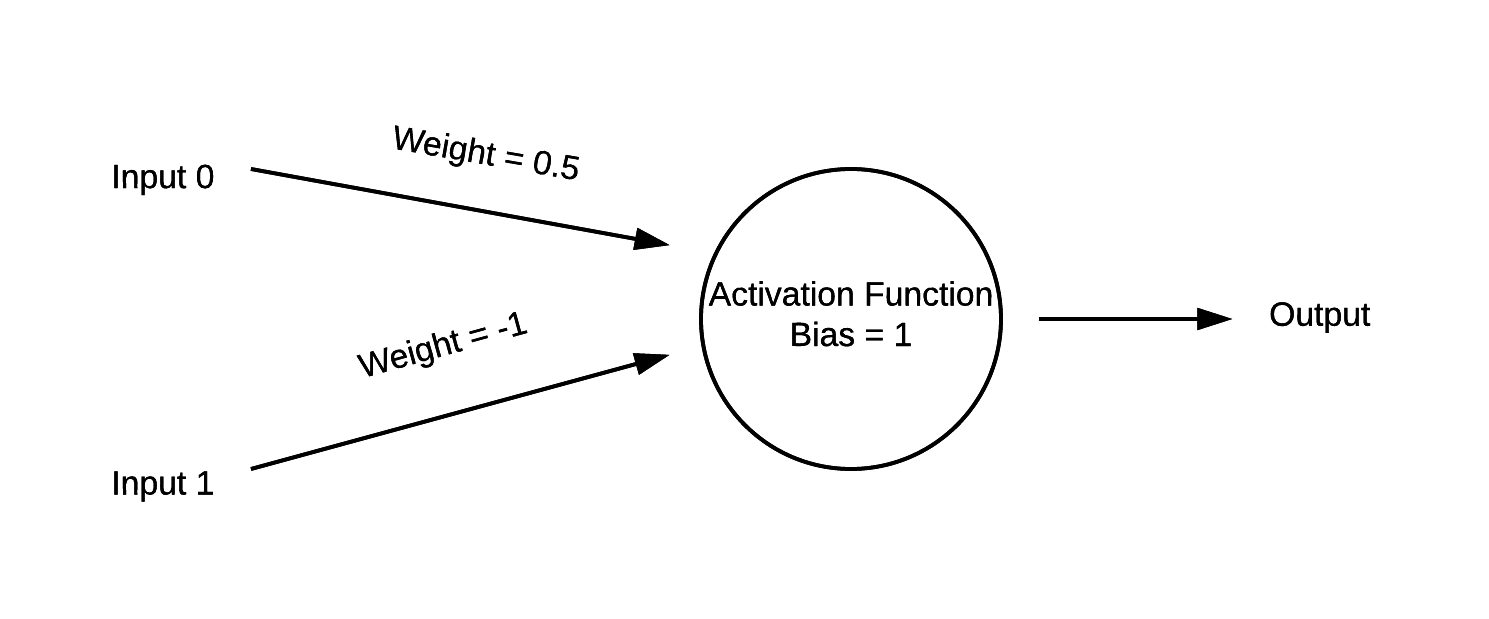
\includegraphics{Perceptron}
     \caption{Perceptron}
     \label{fig:perceptron}
\end{figure}

The Perceptron Training Rule is how weights are selected to produce the correct output during training.
As in \parencite{MLANN}, a common way to train a perceptron is to start with random weights and change them during training as per the training rule.
This rule follows the formula in Equation \ref{eqn:perceptron1}, where xi is the input and Equation \ref{eqn:perceptron2} is valid:
\begin{equation}\label{eqn:perceptron1}
    w_{i} \leftarrow w_{i} + \Delta w_{i}
\end{equation}

\begin{equation}\label{eqn:perceptron2}
    \Delta w_{i} = n(t-o)x_{i}
\end{equation}

In Equation \ref{eqn:perceptron2}, "t is the target output for the current training example, o is the output generated by the perceptron, and n is the positive constant called the learning rate" \parencite{MLANN}.
The output of a neuron is calculated using the activation function.
This Perceptron Training Rule assumes that there are two sets of instances, a
positive and negative set (class x and - in Figure \ref{fig:ls}), and that they are linearly separable, as in demonstrated in Figure \ref{fig:ls}. 

\begin{figure}[h]
	\centering
    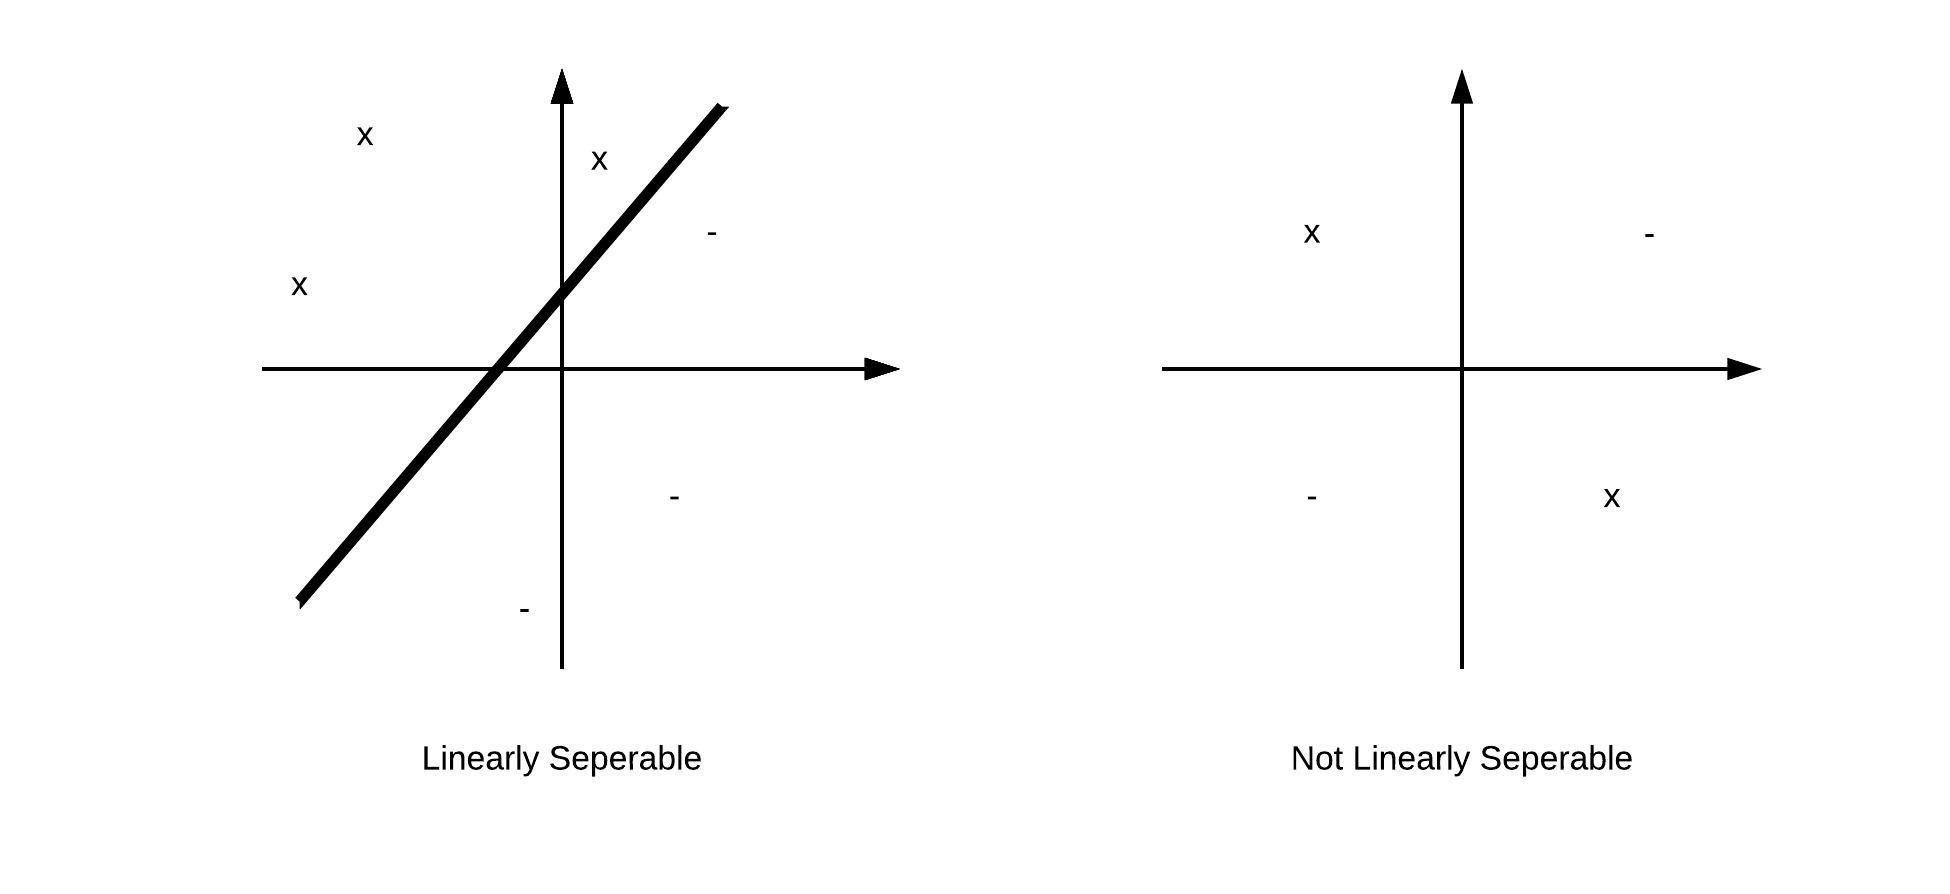
\includegraphics{LS}
     \caption{Linearly Separable, adapted from \parencite{MLANN}}
     \label{fig:ls}
\end{figure}

A perceptron is trained using supervised learning. When the perceptron
classifies a result, it is told if it is correct or not. If the result is
incorrect, weights are changed in value so that this error can be reduced
\parencite{AI}. 

There is one major problem with perceptron learning and that is, it can't solve
a problem if there is not a clear linear separation between the classes. There
is a way in which we can attempt to solve this, through the delta rule. The
delta rule utilises gradient descent to find the best weight for the training
samples \parencite{MLANN}. We will discuss gradient descent in the next section.

\tocless\subsubsection{Multi Layered Perceptron}
Multi-Layer Perceptrons (MLPs) are made up of multiple layers of perceptrons connected
together and are used to combat non-linearly separable classes.
While the delta rule can solve problems of non-linearity when there are two classes, MLPs can solve non-linearity when there are more than two classes.
Firstly, we have an input layer, followed by one or more hidden layers and then
finally an output layer.
Any ANN with more than three hidden layers is categorised as a deep neural network.

\begin{figure}[h]
	\centering
    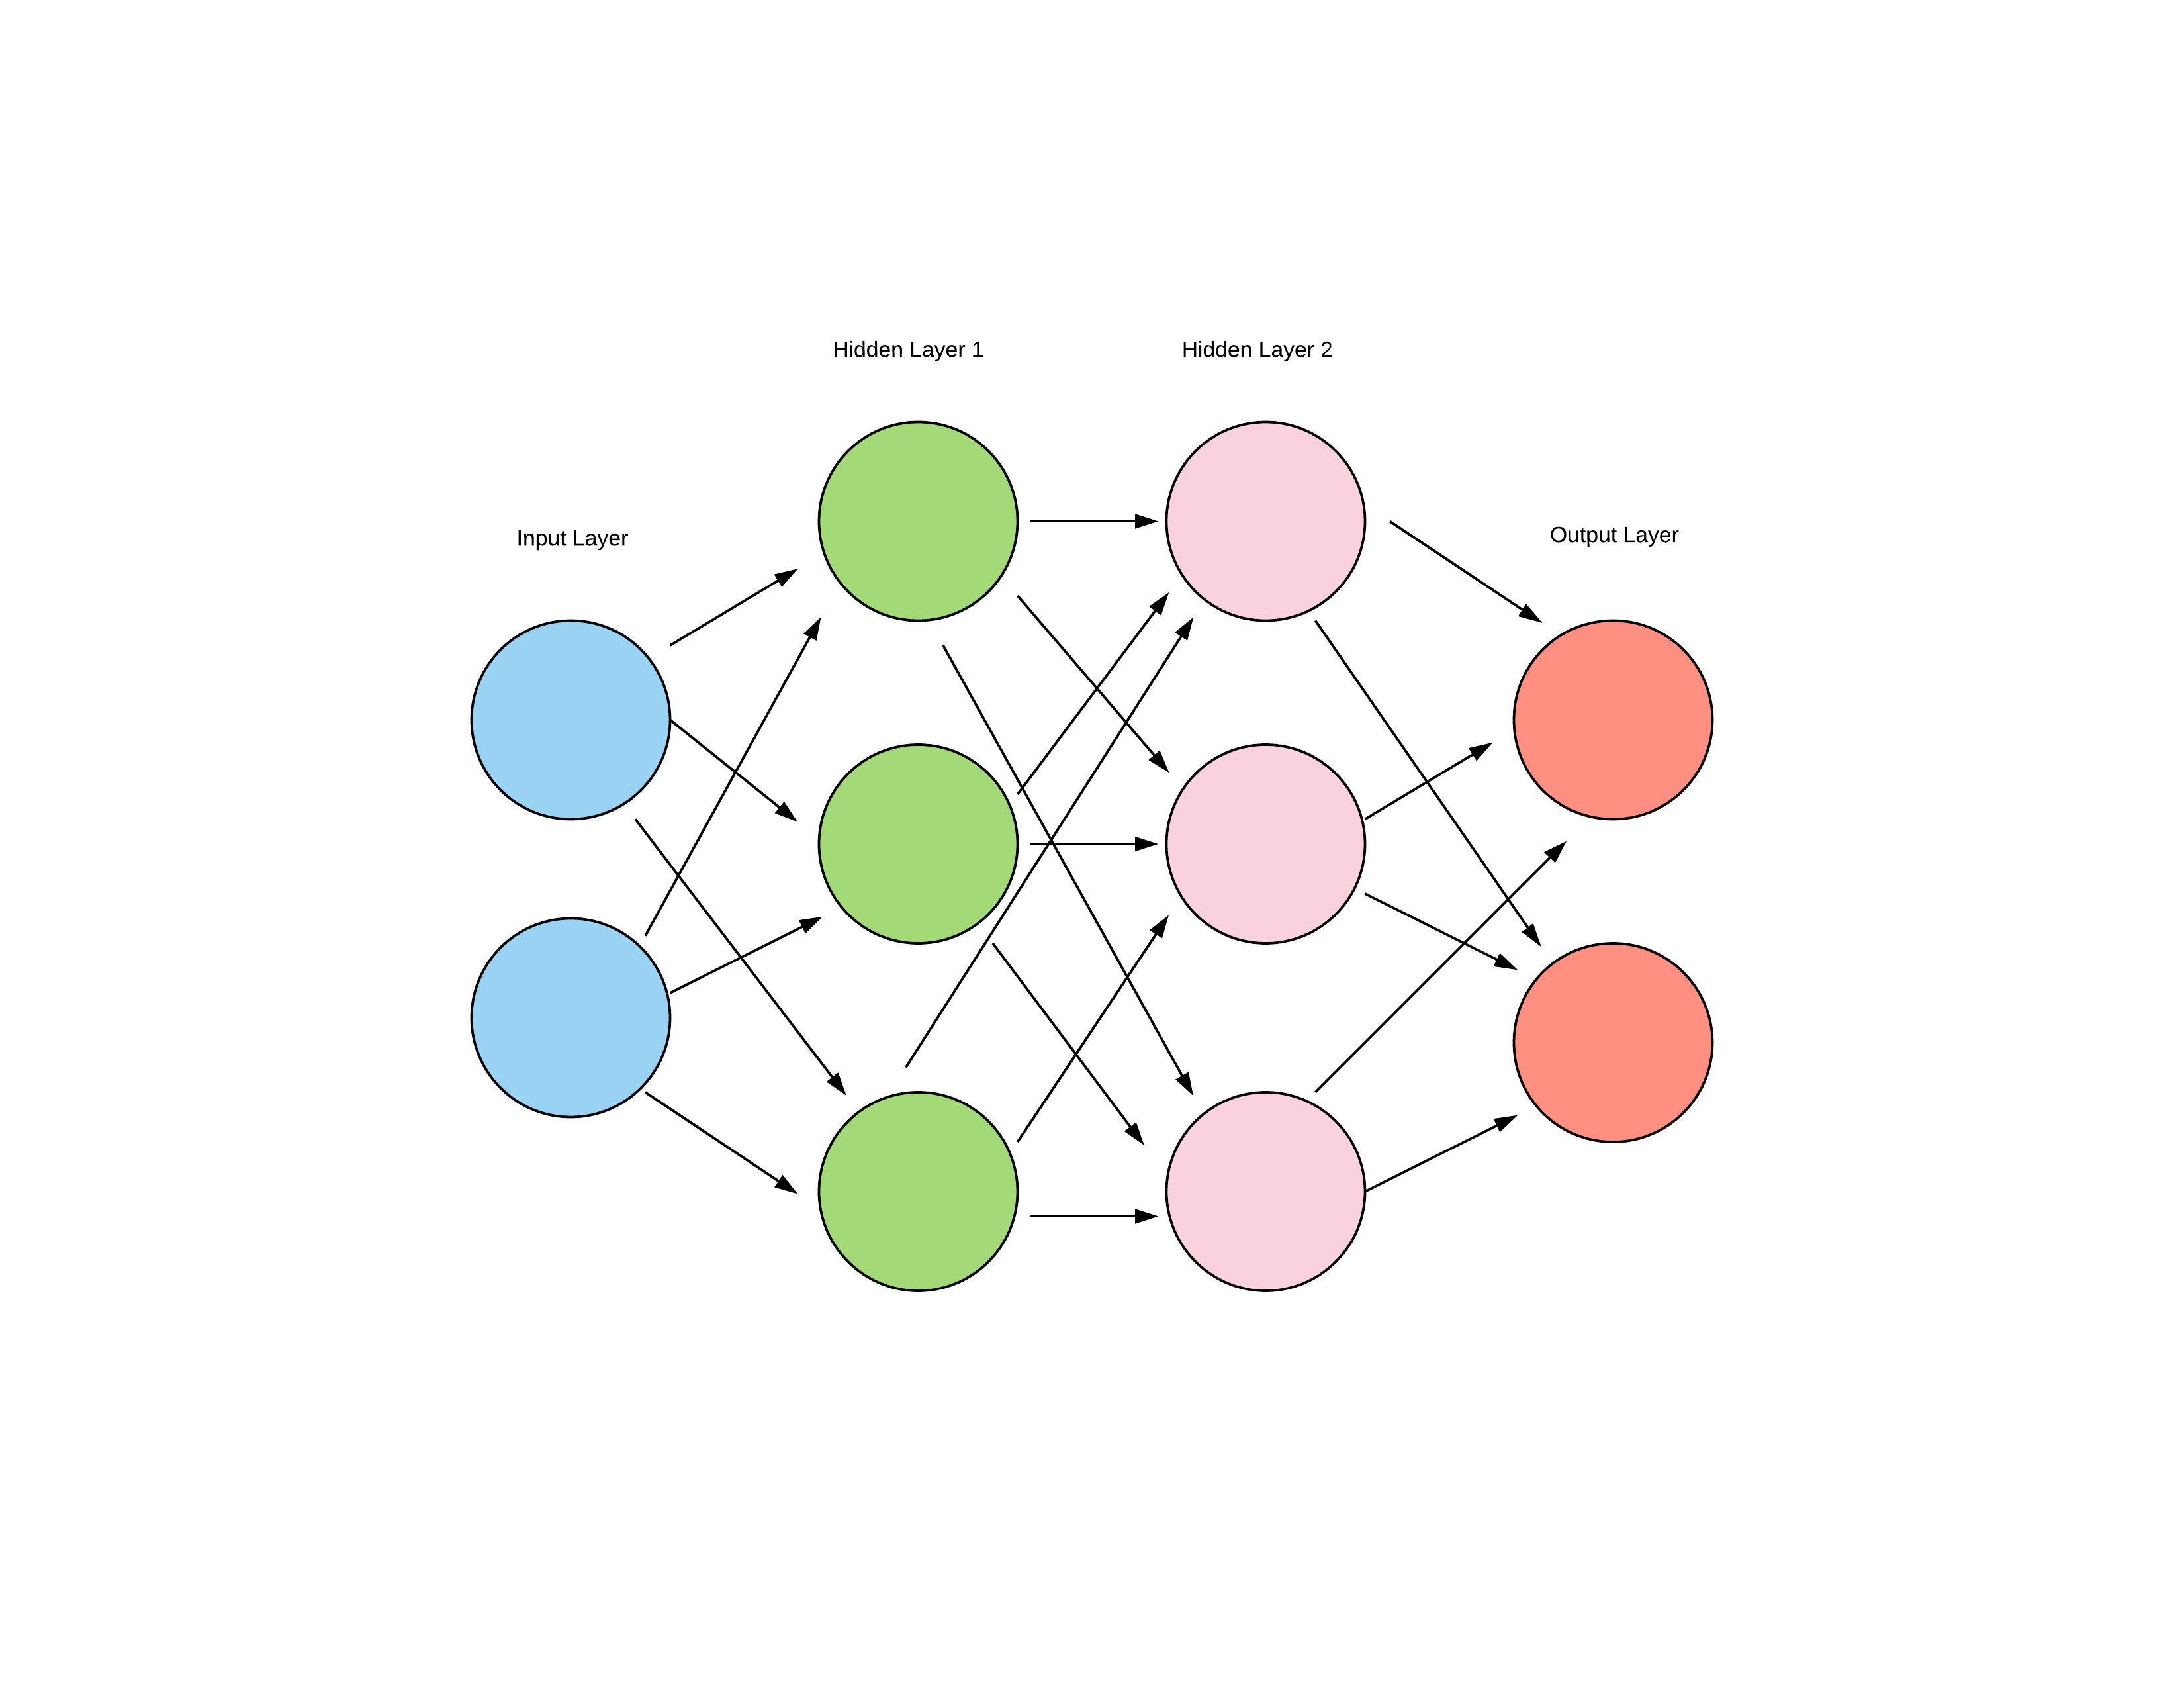
\includegraphics[width=150mm,scale=0.5]{mlp}
    \caption{Multi Layer Perceptron}
    \label{fig:mlp}
\end{figure}

The input layer of a network consists of the data that is fed into the network to be classified. The input layer passes this data to a hidden layer
whose purpose is to transform this data into something that the output layer can
understand. This transformation results in a linearly separable space that can be classified. The output layer normally consists of a class prediction.

MLPs are a class of feed forward ANNs.
These means that the output of each perceptron feeds into an input in the next
layer of the network, example seen in Figure \ref{fig:mlp}.

During training, using backpropagation for each step, the output of every neuron is calculated in each layer and then passed to the next layer. Then the error of the output is calculated, and the network calculates how each neuron in the last hidden layer effected the error. This is continued back through all the layers until the input layer \parencite{handsOnML}. The weights are then altered to try and reduce this error.

There is one large problem with MLP's and as a result CNNs were created. If one is attempting to classify images with a MLP then
each pixel in that image would have to be a separate input. This creates a
massive number of neurons through all the layers and this isn't feasible. CNN's
solve this problem which we will discuss later.



\tocless\subsubsection{Gradient Descent and backpropagation}
Gradient descent is an algorithm used to find the optimal weights to produce the
smallest prediction error. It is used to overcome problems of non-linearly
separable classes. Gradient descent search selects a random weight value and
then modifies it gradually to minimize the error. "At each step, the weight
vector is altered in the direction that produces the steepest descent along the
surface" \parencite{MLANN}. This step is iterated until the lowest value is met.

There is an error function used for the perceptron which finds the lowest error for that neuron, but it can't be used here because, since we have many neurons, there could be an error in multiple neurons.
Gradient descent is mathematically based on the derivative of a function.
The gradient of a function can be calculated by differentiating it.
As the weights are what is being controlled, "they are what we differentiate in respect to" \parencite{MLAlgorithm}.
The negative gradient of this function is followed to find the lowest possible point, hence the name gradient descent \parencite{MLAlgorithm}.

One problem with gradient descent is that if we look at Figure \ref{fig:GD}, we may
never get to the optimal point, point B. This is because we will find point A
without too many problems but when the weights change we will get too high a
slope of error and therefore will never reach point B.

Another variation of gradient descent is Stochastic Gradient Descent (SGD). SGD
is different because it updates "weights incrementally, following the
calculation of the error of each individual example" \parencite{MLANN}. 

\begin{figure}[h]
      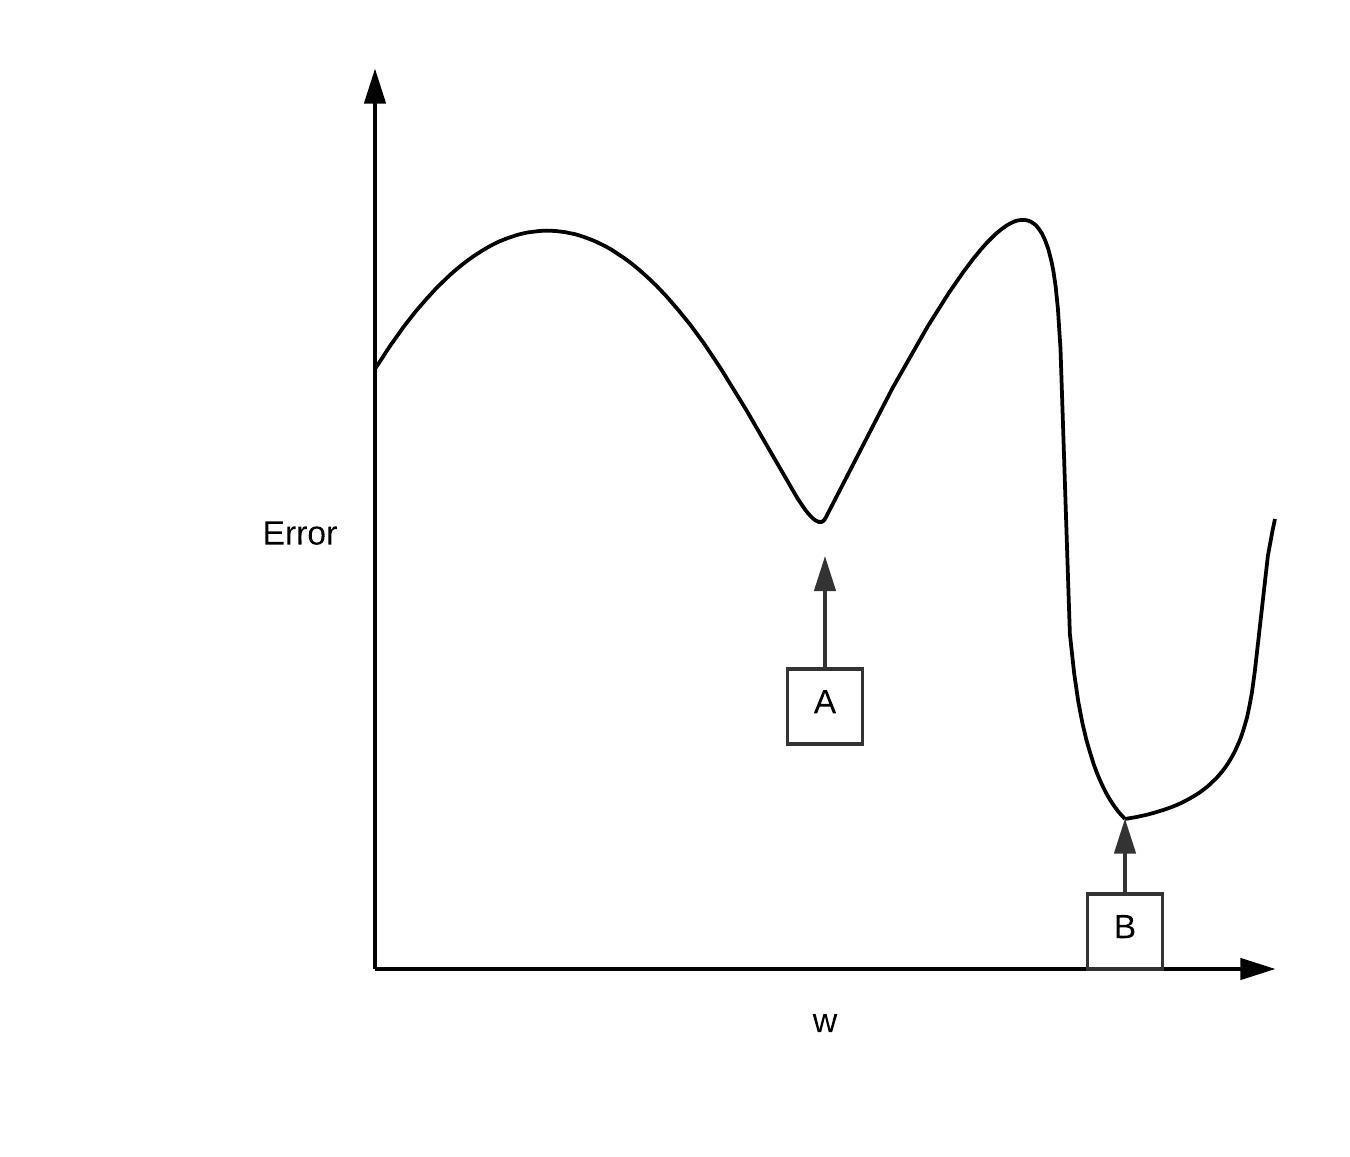
\includegraphics{GradientDescent}
      \caption{Gradient Descent}
      \label{fig:GD}
 \end{figure}

"The Backpropagation algorithm learns the weights of a multilayer network,
given a network with a fixed set of units and interconnections" \parencite{MLANN}.
Backpropagation attempts to minimize the mean squared error between the target
output and the actual output of a network.

Backpropagation works by starting at the output layer of the network and going
back through previous hidden layers, updating weights as it goes i.e. it propagates back through the network, updating the weights to try and reduce the error.

\parencite{MLANN} defined a walkthrough of the backpropagation algorithm.
For every value of Equation \ref{eqn:bp1}, in the training set where x is a vector of inputs and t is a vector of output values to act as a target:
\begin{itemize}
	\item{Run x through the network and output Equation \ref{eqn:bp2}.}
	\item{For each output k, calculate the error by Equation \ref{eqn:bp3}.}
	\item{For every hidden unit, calculate the error by Equation \ref{eqn:bp4}.}
	\item{Update weights by Equation \ref{eqn:bp5} where Equation \ref{eqn:bp5} is true.}
\end{itemize}

\begin{equation}\label{eqn:bp1}
    \vec{x}, \vec{t}
\end{equation}

\begin{equation}\label{eqn:bp2}
    o_{u}
\end{equation}

\begin{equation}\label{eqn:bp3}
    \delta_{k} \leftarrow o_{k}(1 - o_{k})(t_{k} - o_{k}) 
\end{equation}

\begin{equation}\label{eqn:bp4}
    \delta_{h} \leftarrow o_{h}(1 - o_{h}) \sum_{k \in outputs}   w_{kh}\delta_{k}
\end{equation}

\begin{equation}\label{eqn:bp5}
    w_{ji} \leftarrow w_{ji} + \Delta w_{ji}
\end{equation}

\begin{equation}\label{eqn:bp6}
    \Delta w_{ji} = \delta_{j} x_{ji}
\end{equation}
